% Generated by AP Math GOLD PILOT deterministic Python generator.
% input id: H01_circle_tangent_lines
\documentclass{article}
\usepackage[margin=1cm]{geometry}
\def\pgfsysdriver{pgfsys-dvisvgm.def}
\usepackage{fontspec}
\setmainfont{Malgun Gothic}
\setsansfont{Malgun Gothic}
\usepackage{amsmath}
\usepackage{amssymb}
\usepackage{pgfplots}
\pgfplotsset{compat=1.18}
\pagestyle{empty}
\begin{document}
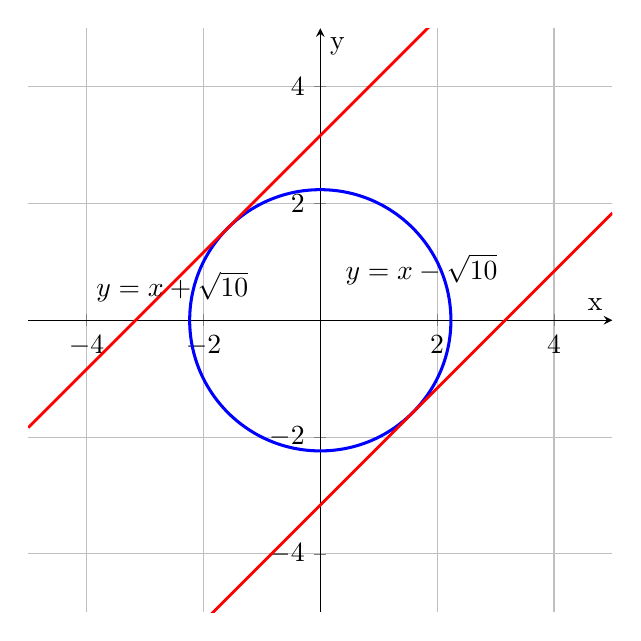
\begin{tikzpicture}
\begin{axis}[width=13cm,height=9cm,axis equal image,axis lines=middle,grid=major,xmin=-5,xmax=5,ymin=-5,ymax=5,xlabel={x},ylabel={y},clip=true]
\draw[blue, solid, line width=1.1pt] (axis cs:0,0) circle [radius=2.236068];
\addplot[red, solid, line width=1pt] coordinates {(-5,-1.837722) (-4.9125,-1.750222) (-4.825,-1.662722) (-4.7375,-1.575222) (-4.65,-1.487722) (-4.5625,-1.400222) (-4.475,-1.312722) (-4.3875,-1.225222) (-4.3,-1.137722) (-4.2125,-1.050222) (-4.125,-0.962722) (-4.0375,-0.875222) (-3.95,-0.787722) (-3.8625,-0.700222) (-3.775,-0.612722) (-3.6875,-0.525222) (-3.6,-0.437722) (-3.5125,-0.350222) (-3.425,-0.262722) (-3.3375,-0.175222) (-3.25,-0.087722) (-3.1625,-0.000222) (-3.075,0.087278) (-2.9875,0.174778) (-2.9,0.262278) (-2.8125,0.349778) (-2.725,0.437278) (-2.6375,0.524778) (-2.55,0.612278) (-2.4625,0.699778) (-2.375,0.787278) (-2.2875,0.874778) (-2.2,0.962278) (-2.1125,1.049778) (-2.025,1.137278) (-1.9375,1.224778) (-1.85,1.312278) (-1.7625,1.399778) (-1.675,1.487278) (-1.5875,1.574778) (-1.5,1.662278) (-1.4125,1.749778) (-1.325,1.837278) (-1.2375,1.924778) (-1.15,2.012278) (-1.0625,2.099778) (-0.975,2.187278) (-0.8875,2.274778) (-0.8,2.362278) (-0.7125,2.449778) (-0.625,2.537278) (-0.5375,2.624778) (-0.45,2.712278) (-0.3625,2.799778) (-0.275,2.887278) (-0.1875,2.974778) (-0.1,3.062278) (-0.0125,3.149778) (0.075,3.237278) (0.1625,3.324778) (0.25,3.412278) (0.3375,3.499778) (0.425,3.587278) (0.5125,3.674778) (0.6,3.762278) (0.6875,3.849778) (0.775,3.937278) (0.8625,4.024778) (0.95,4.112278) (1.0375,4.199778) (1.125,4.287278) (1.2125,4.374778) (1.3,4.462278) (1.3875,4.549778) (1.475,4.637278) (1.5625,4.724778) (1.65,4.812278) (1.7375,4.899778) (1.825,4.987278) (1.9125,5.074778) (2,5.162278)};
\addplot[red, solid, line width=1pt] coordinates {(-2,-5.162278) (-1.9125,-5.074778) (-1.825,-4.987278) (-1.7375,-4.899778) (-1.65,-4.812278) (-1.5625,-4.724778) (-1.475,-4.637278) (-1.3875,-4.549778) (-1.3,-4.462278) (-1.2125,-4.374778) (-1.125,-4.287278) (-1.0375,-4.199778) (-0.95,-4.112278) (-0.8625,-4.024778) (-0.775,-3.937278) (-0.6875,-3.849778) (-0.6,-3.762278) (-0.5125,-3.674778) (-0.425,-3.587278) (-0.3375,-3.499778) (-0.25,-3.412278) (-0.1625,-3.324778) (-0.075,-3.237278) (0.0125,-3.149778) (0.1,-3.062278) (0.1875,-2.974778) (0.275,-2.887278) (0.3625,-2.799778) (0.45,-2.712278) (0.5375,-2.624778) (0.625,-2.537278) (0.7125,-2.449778) (0.8,-2.362278) (0.8875,-2.274778) (0.975,-2.187278) (1.0625,-2.099778) (1.15,-2.012278) (1.2375,-1.924778) (1.325,-1.837278) (1.4125,-1.749778) (1.5,-1.662278) (1.5875,-1.574778) (1.675,-1.487278) (1.7625,-1.399778) (1.85,-1.312278) (1.9375,-1.224778) (2.025,-1.137278) (2.1125,-1.049778) (2.2,-0.962278) (2.2875,-0.874778) (2.375,-0.787278) (2.4625,-0.699778) (2.55,-0.612278) (2.6375,-0.524778) (2.725,-0.437278) (2.8125,-0.349778) (2.9,-0.262278) (2.9875,-0.174778) (3.075,-0.087278) (3.1625,0.000222) (3.25,0.087722) (3.3375,0.175222) (3.425,0.262722) (3.5125,0.350222) (3.6,0.437722) (3.6875,0.525222) (3.775,0.612722) (3.8625,0.700222) (3.95,0.787722) (4.0375,0.875222) (4.125,0.962722) (4.2125,1.050222) (4.3,1.137722) (4.3875,1.225222) (4.475,1.312722) (4.5625,1.400222) (4.65,1.487722) (4.7375,1.575222) (4.825,1.662722) (4.9125,1.750222) (5,1.837722)};
\node[anchor=north west] at (axis cs:-4,1) {$y=x+\sqrt{10}$};
\node[anchor=north east] at (axis cs:3.2,1.3) {$y=x-\sqrt{10}$};
\end{axis}
\end{tikzpicture}
\end{document}
